%% Los cap'itulos inician con \chapter{T'itulo}, estos aparecen numerados y
%% se incluyen en el 'indice general.
%%
%% Recuerda que aqu'i ya puedes escribir acentos como: 'a, 'e, 'i, etc.
%% La letra n con tilde es: 'n.

\chapter{Introducci'on}

\section{Resumen}

\section{Estados ligados en el continuo}

Para entender el interés por construir estados ligaodos en el continuo, empezaremos por establecer la diferencia entre estados ligados y estados de dispersión desde un punto de un sistema mecánico. En mecánica clásica, el movimiento de una partícula con masa $m$ sometido a un potencial $V$ puede ser analizado en términos de la energía mecánica del sistema

\begin{equation}
	E = \frac{1}{2} mv^2 + V, \label{EM}
\end{equation}

donde (\ref{EM})  se puede escribir a su vez en términos de la velocidad de la partícula en la forma

\begin{equation*}
v = \sqrt{\frac{2(E-V)}{m}},
\end{equation*}

lo cual permite observar que para el caso $E < V$, el término dentro de la raíz es negativa y la velocidad puramente imaginaria,lo cual no tiene significado físico. Como consecuencia, existirán zonas $"$prohibidas$"$ en el espacio donde el cuerpo no podrá desplazarse. Tenemos entonces tres casos principales para el desplazamiento de la partícula (ver figura \ref{Ex-Pot-Figure}), distinguibles en términos de los puntos donde $V(x_r) = E$. Los puntos $x_r$ son conocidos como puntos de retorno, ya que definen el momento donde $v=0$ y el movimiento cambia de dirección. 

El primer caso es aquel donde la partícula se encuentra en una región acotada por dos puntos de retorno clásico, por lo que sólo podrá desplazarse en una zona finita del espacio, es decir, la partícula estará confinada ($E_1$, $E_2$).

Si la patícula se encuentra en una región acotada por un sólo punto de retorno, esto quiere decir que aunque el movimiento de la partícula está restringido, la región donde puede desplazarse no es finita y por lo tanto no hay confinamiento ($E_3$).

Finalmente, si la energía de la partícula es siempre mayor al potencial, ésta podrá desplazarse por todo el espacio, sólo experimentando cambios en su velocidad debido a variaciones en su energía cinética ($E_4$). 

Podemos concluir entonces que para tener confinamiento en mecánica clásica es una condición necesaria y suficiente que la partícula se enciuentre en una región acotada por dos puntos de retirno clásico. A continuación veremos como esta condición ya no es suficiente a la hora de hablar de confinamiento en mecánica cuántica.

 
En mecánica cuántica, la ley dinámica que describe el comportamiento de un sistema es la ecuación de Scrödinger, la cual en su representación de coordenadas es

\begin{equation}
	-\frac{\hbar^2}{2m}  \frac{\partial^2 \Psi}{\partial x^2}+ V(x) \Psi = i\hbar \frac{\partial \Psi}{\partial t}\label{ES1D},
\end{equation}
la cual puede ser vista como un análogo de la ecuación (\ref{EM}), en términos de operadores actuando sobre una función $\psi$, que permite obtener la densidades de probabilidad a través de su módulo al cuadrado, dándole el carácter predictivo a la teoría. Por lo tanto, la siguiente condición a la frontera se debe satisfacer

\begin{equation*}
	\int_{\mathbb{R}} |\Psi|^2 d^3 x \label{CFP}
\end{equation*}

Para resolver (\ref{ES1D}), proponemos que la función de onda $\Psi$ sea de la forma


\begin{equation*}
	\Psi(x,t) = \psi(x) \phi(t)
\end{equation*}

por lo que al dividir ambos lados de (\ref{ES1D}) entre $\Psi$ se obtiene

\begin{equation*}
-\frac{\hbar^2}{2m}  \frac{1}{\psi}\frac{\partial^2 \psi}{\partial x^2}+ V(x) \psi= i\hbar \frac{1}{\phi}\frac{\partial \phi}{\partial t}.
\end{equation*}

Como ambos lados de esta ecuación dependen de una sola variable, ésta se puede desacoplar igualando cada lado a una constante $E$

\begin{eqnarray*}
	-\frac{\hbar^2}{2m}  \frac{d^2 \psi}{d x^2}+ V(x) \psi = E \psi
	\\
	 \frac{d \phi}{dt} = -i \frac{E}{\hbar} \phi
\end{eqnarray*}

por lo que el problema se reduce a resolver la primer ecuación para una función $V(x)$ específica. 

Finalmente, debido a que se debe satisfacer de alguna manera la condición (\ref{CFP}), las soluciones a la ecuación de Schrödinger con significado físico son evidentemente las funciones de cuadrado integrable y las funciones acotadas, ya que aunque no cumplen directamente con la condición a la frontera, se pueden usar para construir un paquete de ondas que si la satisface (ver figura \ref{WP-Figure}).  
\begin{figure}
	\begin{center}
		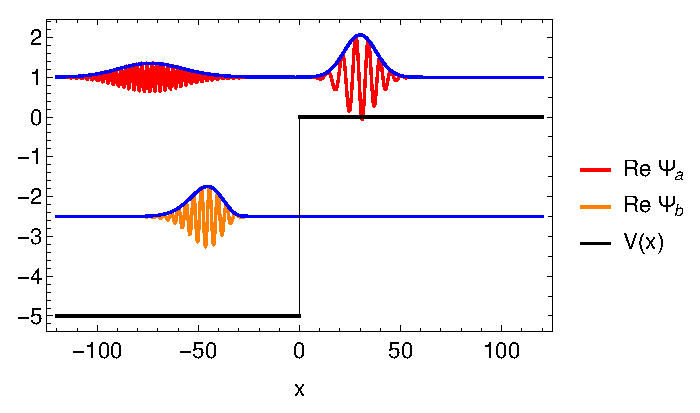
\includegraphics{WP.eps}%
	\end{center}	
	\caption{\label{WP-Figure} Paquete de ondas dispersado por una barrera de potencial $V(x)$. Si la energía se encuentra por debajo del umbral, la totalidad del paquete será reflejada ($\Psi_b$), en caso contrario, sólo parte del paquete será transmitida ($\Psi_a$).}
\end{figure}

Este resultado permite establecer la diferencia clave entre un sistema goberando por la mecánica cúantica con respecto al caso de un sistema cásico sometido al mismo potencial, en este caso ilustrado por \ref{Ex-Pot-Figure}. Debido a la naturaleza estadística de la función de onda, en un sistema cuántico existirá la posibilidad de que la partícula se encuentre en una zona prohibida clásicamente, lo que se conoce como efecto túnel. Sin embargo, en el caso de las funciones de cuadrado integrable, llamadas estados ligados, seguirá siendo posible el confinamiento, en este caso, de la función de onda. Por otro lado, para el caso de un ente cuántico descrito por una función acotada, llamado estado de dispersión, este podrá ser reflejado por el potencial a pesar de que su energía sea mayor a la del potencial. La probabilidad de que esto ocurra esta dada por los coeficientes de transmisión y reflexión.  

Podemos concluir entonces  debido al efecto túnel, en un sistema cuántico no es suficiente la existencia de dos puntos de retorno clásico para que exista confinamiento, si no que además se debe garantizar que las berreras de potencial a las que este sometida la partícula sean de ancho infinito, es decir

\begin{equation*}
	\lim_{|x|\to \infty} V(x) > E \label{CEL}
\end{equation*}

Sin embargo, el hecho de que una función de onda pueda ser reflejada por el potencial sugiere que se puede construir un potencial cuyo efecto sobre la transmisión y reflexión de la función de onda sea tal que esta se pueda confinar a pesar de que su enenrgía no cumpla con (\ref{CEL}) . Estos estados fueron propuestos por von Neumann y Wigner en 1939, siendo llamados estados ligados en el continuo debido a que son funciones de cuadrado integrable con un valor de la energía convencionalemente asociada al espectro de dispersión, el cual es continuo. En la siguiente subsección se desarrollará el método usado para concebir estos peculiares estados.


\begin{figure}
	\begin{center}
		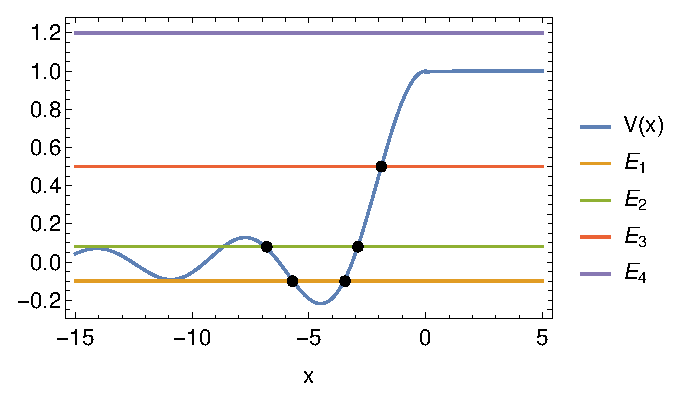
\includegraphics{Ex-Pot.eps}%
	\end{center}	
	\caption{\label{Ex-Pot-Figure} Ejemplo de de un una sistema mecánico sometido a un potencial para diferentes valores de la energía 
	}
\end{figure}


\section{Potenciales de von Neumann Wigner}
\subsection{Método de von Neumann Wigner}

El método de von Neumann - Wigner se basa en ver un problema de la mecánica cuántica de una manera diferente a la habitual. Mediante la ecuación de Schrödinger radial con momento angular cero con unidades adecuadas 

\begin{equation*}
	-\frac{1}{2} \nabla^2 \psi + V(r) \psi = E \psi
\end{equation*}  

podemos encontrar el potencial a través de proponer que la eigenfunción para la energía $E = \frac{k^2}{2}$ sea de la forma de una solución al problema de partícula libre modulada por una función $f(r)$

\begin{eqnarray}
	\label{MvNW-V}
	V(r)  = E + \frac{1}{2} \frac{\nabla^2 \psi}{\psi} 
	\\
	\label{MvNW-Psi}
	\psi = f(r) \frac{\sin(kr)}{kr}
\end{eqnarray}   

sustituyendo (\ref{MvNW-Psi}) en (\ref{MvNW-V}) y desarrollando la gradiente se llega a una expresión para el potencial en términos de la función de modulación 

\begin{equation*}
	V(r)= k \cot{kr}\,\frac{f'(r)}{f(r)}+\frac{1}{2}\frac{f''(r)}{f(r)}, \quad {\rm donde}\quad '\equiv \frac{d}{dr}.\label{vNW-Vf}.
\end{equation*}

Para asegurar que el sistema resultante tenga espectro de dispersión, necesitamos que el potencial sea acotado, para lo cual los ceros en $\sin{kr}$ y $f(r)$ se deben compensar con los ceros de $f'(r)$ y $f''(r)$ respectivamente. Peoponemos entonces que la derivada de $f(r)$
sea de la forma

\begin{equation*}
f'(r) = g(r)\sin^n(kr)
\end{equation*}

Como caso inmediato, podemos estudiar lo que ocurre para $n=1$ y $g(r)=k$

\begin{equation*}
f'(r) = k \sin(kr) \Rightarrow \,\, 
\begin{matrix}
f(r) = - \cos(kr) & \,
\\
f''(r) = k^2 \cos(kr) & \,
\end{matrix}
\end{equation*}

sustituyendo en el potencial, éste se reduce a

\begin{equation*}
V(r)= -\frac{3}{2}k^2,
\end{equation*}

el cual no es más que el potencial de partícula libre desplazado, por lo que este caso no es de utilidad. Analicemos lo que ocurre para $n=2$ y $g(r)=k$, entonces

\begin{equation*}
f'(r) = k \sin^2(kr) \Rightarrow \,\, 
\begin{matrix}
f(r) = \frac{2 k r-\sin(2kr)}{4} & \,
\\
f''(r) = 2 k^2 \sin(kr) \cos(kr) & \,
\end{matrix}
\end{equation*}

por lo que el potencial es de la forma

\begin{equation*}
	V(r)=\frac{16 k^2 \sin(2kr)}{2 k r-\sin(2kr)}.
\end{equation*}

En este caso, hemos obtenido un potencial acotado, sin embargo, la función de onda queda de la forma

\begin{equation*}
\psi(k,r)=\frac{[2 k r-\sin(2kr)]\sin(kr)}{4 k r},
\end{equation*}

pr lo que asintóticamente, esta función va como $\sin(kr)$, por lo que no es una función de cuadrado integrable. 

A pesar  de no haber obtenido una solución de la forma deseada en el análisis anterior, podemos modificarlo proponiendo una función de modulación de la forma de una composición de funciones, lo que permite usar la regla de la cadena para obtener su derivada

\begin{equation*}
f(r) = f(h(r)) \Rightarrow f'(r) = \frac{dh}{dr} \frac{df}{dh} 
\end{equation*}

donde las respectivas funciones son

\begin{eqnarray*}
f(r) &=& \frac{1}{A^2 - 16h^2(r)}
\\
h(r) &=& \frac{2 k r-\sin(2kr)}{4},
\end{eqnarray*}

donde $A$ es una costante real cuyo propósito es evitar que el denominador de $f(r)$ cause singularidades tanto en el potencial como en las función de onda. Además, podemos observar que $h(r)$ es de la misma forma que $f(r)$ en el caso anterior, por lo que

\begin{equation*}
\frac{dh}{dr} =  k \sin^2(kr).
\end{equation*}

La función de modulación tiene finalmente la forma requerida. Más aún, la función de onda resulta ser de la forma 
\begin{equation*}
	\psi(r) = \frac{\sin(kr)}{k r \{A^2 - [2 k r-\sin(2kr)]^2\}}.
\end{equation*}

Como ésta es una función con una envolvente que va como $\frac{1}{r^3}$, es una función de cuadrado integrable.

Lo único que resta es obtener la forma del potencial por mmedio de la fórmula (\ref{vNW-Vf}), donde los ceros de $\sin(kr)$ han sido compensados por la forma de $f(r)$, y ya que ésta misma carece de ceros, no es necesario analizar los otros dos términos. El potencial está dado por la expresión analítica

\begin{eqnarray*}
	V(r)&=&-\frac{64 k^2 A^2 \sin^4(kr)}{\{A^2 + [2kr - \sin(2kr)]^2\}^2}
	\\
	 &+& \frac{48 k^2 \sin^4(kr) - 8 k^2[2kr - \sin(2kr)]\sin(2kr)}{A^2 + [2kr - \sin(2kr)]^2}
\end{eqnarray*}


y se puede escribir de acuerdo a su comportamiento como

\begin{equation}
	V(r) = a\,\frac{\sin{br}}{r}+ O\left(\frac{1}{r^2}\right).\label{vNW-V2}
\end{equation}

donde $b = 2 k$ y $a = 4 k^2$. En trabajos posteriores, se demostró que los potenciales de la forma \ref{vNW-V2} pueden alojar un estado ligado en el continuo en $E = \frac{b^2}{4}$, siempre que   $|b| <|a|$. La figura \ref{vNW-Figure} muestra el gráfico de un potencial creado mediante este método. 

Aúnque se ha demostrado que matemáticamente se pueden construir sistemas que admitan estados ligados en el continuo, el sistema creado por método presentado en esta sección tiene dos importantes limitantes. La primera es de índole matemática y se debe a que sólo se puede conocer de menera análitica una de sus soluciones, que es precisamente squella correspondiente al estado ligado en el continuo. La segunda y más importante se encuentra en la física, ya que no se ha enconrado en la naturaleza un potencial que se comporte de esta manera. Por consiguiete, se han propuesto métodos para la construcción de sistemas cuánticos solubles, en donde uno de los más populares es la transformación de Darboux, la cual estudiaremos en la siguiente sección.

\begin{figure}
	\begin{center}
		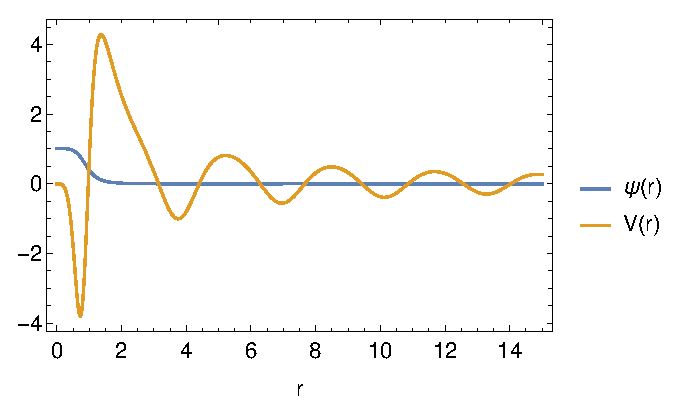
\includegraphics[scale=0.6]{vNW-Figure.eps}
	\end{center}
	\caption{\label{vNW-Figure} \footnotesize Potencial de von Neumann - Wigner(línea punteada) y su correspondiente estado ligado en el cpntinuo (línea sólida) para $k=1$ y $A=1$.}
\end{figure}



